\documentclass[margin = 1pt, tikz]{standalone}
\usepackage{tikz}
\usepackage{bm}
\usepackage{relsize}

\usetikzlibrary{arrows.meta}

\usetikzlibrary{positioning}

% COLORS
\usepackage{xcolor}
\colorlet{myred}{red!80!black}
\colorlet{myblue}{blue!80!black}
\colorlet{mybluee}{myblue!80!black}
\colorlet{mygreen}{green!60!black}
\colorlet{myorange}{orange!70!red!60!black}
\colorlet{mydarkred}{red!30!black}
\colorlet{mydarkblue}{blue!40!black}
\colorlet{mydarkgreen}{green!30!black}

\begin{document}
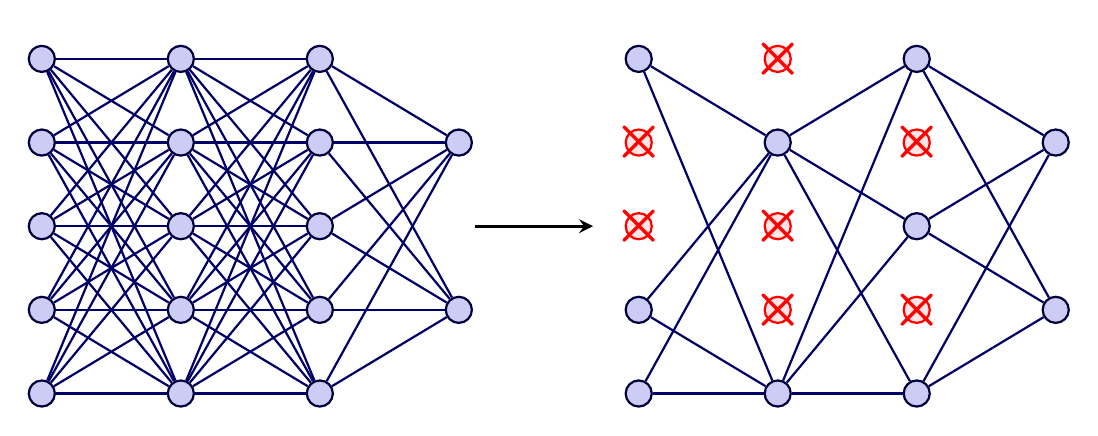
\begin{tikzpicture}

	\node[circle, draw, thick, blue!20!black,draw=myblue!30!black,fill=myblue!20, blue!20!black,draw=myblue!30!black,fill=myblue!20] (i1) {};
	\node[circle, draw, thick, blue!20!black,draw=myblue!30!black,fill=myblue!20, above=2em of i1] (i2) {};
	\node[circle, draw, thick, blue!20!black,draw=myblue!30!black,fill=myblue!20, above=2em of i2] (i3) {};
	\node[circle, draw, thick, blue!20!black,draw=myblue!30!black,fill=myblue!20, below=2em of i1] (i4) {};
	\node[circle, draw, thick, blue!20!black,draw=myblue!30!black,fill=myblue!20, below=2em of i4] (i5) {};
	
	\node[circle, draw, thick, blue!20!black,draw=myblue!30!black,fill=myblue!20, right=4em of i1] (h1) {};
	\node[circle, draw, thick, blue!20!black,draw=myblue!30!black,fill=myblue!20, right=4em of i2] (h2) {};
	\node[circle, draw, thick, blue!20!black,draw=myblue!30!black,fill=myblue!20, right=4em of i3] (h3) {};
	\node[circle, draw, thick, blue!20!black,draw=myblue!30!black,fill=myblue!20, right=4em of i4] (h4) {};
	\node[circle, draw, thick, blue!20!black,draw=myblue!30!black,fill=myblue!20, right=4em of i5] (h5) {};
	
	\node[circle, draw, thick, blue!20!black,draw=myblue!30!black,fill=myblue!20, right=4em of h1] (hh1) {};
	\node[circle, draw, thick, blue!20!black,draw=myblue!30!black,fill=myblue!20, right=4em of h2] (hh2) {};
	\node[circle, draw, thick, blue!20!black,draw=myblue!30!black,fill=myblue!20, right=4em of h3] (hh3) {};
	\node[circle, draw, thick, blue!20!black,draw=myblue!30!black,fill=myblue!20, right=4em of h4] (hh4) {};
	\node[circle, draw, thick, blue!20!black,draw=myblue!30!black,fill=myblue!20, right=4em of h5] (hh5) {};
	
	\node[circle, draw, thick, blue!20!black,draw=myblue!30!black,fill=myblue!20, right=4em of hh2] (o1) {};
	\node[circle, draw, thick, blue!20!black,draw=myblue!30!black,fill=myblue!20, right=4em of hh4] (o2) {};
	
	\draw[-, thick, thick,mydarkblue] (i1) -- (h1);
	\draw[-, thick, thick,mydarkblue] (i1) -- (h2);
	\draw[-, thick, thick,mydarkblue] (i1) -- (h3);
	\draw[-, thick, thick,mydarkblue] (i1) -- (h4);
	\draw[-, thick, thick,mydarkblue] (i1) -- (h5);
	\draw[-, thick, thick,mydarkblue] (i2) -- (h1);
	\draw[-, thick, thick,mydarkblue] (i2) -- (h2);
	\draw[-, thick, thick,mydarkblue] (i2) -- (h3);
	\draw[-, thick, thick,mydarkblue] (i2) -- (h4);
	\draw[-, thick, thick,mydarkblue] (i2) -- (h5);
	\draw[-, thick, thick,mydarkblue] (i3) -- (h1);
	\draw[-, thick, thick,mydarkblue] (i3) -- (h2);
	\draw[-, thick, thick,mydarkblue] (i3) -- (h3);
	\draw[-, thick, thick,mydarkblue] (i3) -- (h4);
	\draw[-, thick, thick,mydarkblue] (i3) -- (h5);
	\draw[-, thick, thick,mydarkblue] (i4) -- (h1);
	\draw[-, thick, thick,mydarkblue] (i4) -- (h2);
	\draw[-, thick, thick,mydarkblue] (i4) -- (h3);
	\draw[-, thick, thick,mydarkblue] (i4) -- (h4);
	\draw[-, thick, thick,mydarkblue] (i4) -- (h5);
	\draw[-, thick, thick,mydarkblue] (i5) -- (h1);
	\draw[-, thick, thick,mydarkblue] (i5) -- (h2);
	\draw[-, thick, thick,mydarkblue] (i5) -- (h3);
	\draw[-, thick, thick,mydarkblue] (i5) -- (h4);
	\draw[-, thick, thick,mydarkblue] (i5) -- (h5);
	
	\draw[-, thick, thick,mydarkblue] (h1) -- (hh1);
	\draw[-, thick, thick,mydarkblue] (h1) -- (hh2);
	\draw[-, thick, thick,mydarkblue] (h1) -- (hh3);
	\draw[-, thick, thick,mydarkblue] (h1) -- (hh4);
	\draw[-, thick, thick,mydarkblue] (h1) -- (hh5);
	\draw[-, thick, thick,mydarkblue] (h2) -- (hh1);
	\draw[-, thick, thick,mydarkblue] (h2) -- (hh2);
	\draw[-, thick, thick,mydarkblue] (h2) -- (hh3);
	\draw[-, thick, thick,mydarkblue] (h2) -- (hh4);
	\draw[-, thick, thick,mydarkblue] (h2) -- (hh5);
	\draw[-, thick, thick,mydarkblue] (h3) -- (hh1);
	\draw[-, thick, thick,mydarkblue] (h3) -- (hh2);
	\draw[-, thick, thick,mydarkblue] (h3) -- (hh3);
	\draw[-, thick, thick,mydarkblue] (h3) -- (hh4);
	\draw[-, thick, thick,mydarkblue] (h3) -- (hh5);
	\draw[-, thick, thick,mydarkblue] (h4) -- (hh1);
	\draw[-, thick, thick,mydarkblue] (h4) -- (hh2);
	\draw[-, thick, thick,mydarkblue] (h4) -- (hh3);
	\draw[-, thick, thick,mydarkblue] (h4) -- (hh4);
	\draw[-, thick, thick,mydarkblue] (h4) -- (hh5);
	\draw[-, thick, thick,mydarkblue] (h5) -- (hh1);
	\draw[-, thick, thick,mydarkblue] (h5) -- (hh2);
	\draw[-, thick, thick,mydarkblue] (h5) -- (hh3);
	\draw[-, thick, thick,mydarkblue] (h5) -- (hh4);
	\draw[-, thick, thick,mydarkblue] (h5) -- (hh5);
	
	
	\draw[-, thick, thick,mydarkblue] (hh1) -- (o1);
	\draw[-, thick, thick,mydarkblue] (hh1) -- (o2);
	\draw[-, thick, thick,mydarkblue] (hh2) -- (o1);
	\draw[-, thick, thick,mydarkblue] (hh2) -- (o2);
	\draw[-, thick, thick,mydarkblue] (hh3) -- (o1);
	\draw[-, thick, thick,mydarkblue] (hh3) -- (o2);
	\draw[-, thick, thick,mydarkblue] (hh4) -- (o1);
	\draw[-, thick, thick,mydarkblue] (hh4) -- (o2);
	\draw[-, thick, thick,mydarkblue] (hh5) -- (o1);
	\draw[-, thick, thick,mydarkblue] (hh5) -- (o2);
	
	\draw[-stealth, very thick] (5.5,0) -- node[above] {} (7, 0);
	
	
	\node[circle, draw, thick, blue!20!black,draw=myblue!30!black,fill=myblue!20, red, fill=red!10, right=10.5em of hh1] (i1) {};
	\node[circle, draw, thick, blue!20!black,draw=myblue!30!black,fill=myblue!20, red, fill=red!10, above=2em of i1] (i2) {};
	\node[circle, draw, thick, blue!20!black,draw=myblue!30!black,fill=myblue!20, above=2em of i2] (i3) {};
	\node[circle, draw, thick, blue!20!black,draw=myblue!30!black,fill=myblue!20, below=2em of i1] (i4) {};
	\node[circle, draw, thick, blue!20!black,draw=myblue!30!black,fill=myblue!20, below=2em of i4] (i5) {};
	
	\node[red] (icr) at (i1) {$\mathlarger{\mathlarger{\mathlarger{\mathlarger{\mathlarger{\bm{\times}}}}}}$};
	\node[red] (icr) at (i2) {$\mathlarger{\mathlarger{\mathlarger{\mathlarger{\mathlarger{\bm{\times}}}}}}$};
	
	\node[circle, draw, thick, blue!20!black,draw=myblue!30!black,fill=myblue!20, red, fill=red!10, right=4em of i1] (h1) {};
	\node[circle, draw, thick, blue!20!black,draw=myblue!30!black,fill=myblue!20, right=4em of i2] (h2) {};
	\node[circle, draw, thick, blue!20!black,draw=myblue!30!black,fill=myblue!20, red, fill=red!10, right=4em of i3] (h3) {};
	\node[circle, draw, thick, blue!20!black,draw=myblue!30!black,fill=myblue!20, red, fill=red!10, right=4em of i4] (h4) {};
	\node[circle, draw, thick, blue!20!black,draw=myblue!30!black,fill=myblue!20, right=4em of i5] (h5) {};
	
	\node[red] (icr) at (h1) {$\mathlarger{\mathlarger{\mathlarger{\mathlarger{\mathlarger{\bm{\times}}}}}}$};
	\node[red] (icr) at (h3) {$\mathlarger{\mathlarger{\mathlarger{\mathlarger{\mathlarger{\bm{\times}}}}}}$};
	\node[red] (icr) at (h4) {$\mathlarger{\mathlarger{\mathlarger{\mathlarger{\mathlarger{\bm{\times}}}}}}$};
	
	\node[circle, draw, thick, blue!20!black,draw=myblue!30!black,fill=myblue!20, right=4em of h1] (hh1) {};
	\node[circle, draw, thick, blue!20!black,draw=myblue!30!black,fill=myblue!20, red, fill=red!10, right=4em of h2] (hh2) {};
	\node[circle, draw, thick, blue!20!black,draw=myblue!30!black,fill=myblue!20, right=4em of h3] (hh3) {};
	\node[circle, draw, thick, blue!20!black,draw=myblue!30!black,fill=myblue!20, red, fill=red!10, right=4em of h4] (hh4) {};
	\node[circle, draw, thick, blue!20!black,draw=myblue!30!black,fill=myblue!20, right=4em of h5] (hh5) {};
	
	\node[red] (icr) at (hh2) {$\mathlarger{\mathlarger{\mathlarger{\mathlarger{\mathlarger{\bm{\times}}}}}}$};
	\node[red] (icr) at (hh4) {$\mathlarger{\mathlarger{\mathlarger{\mathlarger{\mathlarger{\bm{\times}}}}}}$};
	
	\node[circle, draw, thick, blue!20!black,draw=myblue!30!black,fill=myblue!20, right=4em of hh2] (o1) {};
	\node[circle, draw, thick, blue!20!black,draw=myblue!30!black,fill=myblue!20, right=4em of hh4] (o2) {};
	
	\draw[-, thick, thick,mydarkblue] (i3) -- (h2);
	\draw[-, thick, thick,mydarkblue] (i3) -- (h5);
	\draw[-, thick, thick,mydarkblue] (i4) -- (h2);
	\draw[-, thick, thick,mydarkblue] (i4) -- (h5);
	\draw[-, thick, thick,mydarkblue] (i5) -- (h2);
	\draw[-, thick, thick,mydarkblue] (i5) -- (h5);
	
	\draw[-, thick, thick,mydarkblue] (h2) -- (hh1);
	\draw[-, thick, thick,mydarkblue] (h2) -- (hh3);
	\draw[-, thick, thick,mydarkblue] (h2) -- (hh5);
	\draw[-, thick, thick,mydarkblue] (h5) -- (hh1);
	\draw[-, thick, thick,mydarkblue] (h5) -- (hh3);
	\draw[-, thick, thick,mydarkblue] (h5) -- (hh5);
	
	\draw[-, thick, thick,mydarkblue] (hh1) -- (o1);
	\draw[-, thick, thick,mydarkblue] (hh1) -- (o2);
	\draw[-, thick, thick,mydarkblue] (hh3) -- (o1);
	\draw[-, thick, thick,mydarkblue] (hh3) -- (o2);
	\draw[-, thick, thick,mydarkblue] (hh5) -- (o1);
	\draw[-, thick, thick,mydarkblue] (hh5) -- (o2);

\end{tikzpicture}
\end{document}